\begin{comment}
\documentclass[10pt]{article}
\usepackage{fullpage, graphicx, url}
\setlength{\parskip}{1ex}
\setlength{\parindent}{0ex}
\title{FLbutBank}
\begin{document}


\begin{tabular}{ccc}
The Alternative Csound Reference Manual & & \\
Previous & &Next

\end{tabular}

%\hline 
\end{comment}
\section{FLbutBank}
FLbutBank�--� A FLTK widget opcode that creates a bank of buttons. \subsection*{Description}


  A FLTK widget opcode that creates a bank of buttons. 
\subsection*{Syntax}


 kout, ihandle \textbf{FLbutBank}
 itype, inumx, inumy, iwidth, iheight, ix, iy, iopcode [, kp1] [, kp2] [, kp3] [, kp4] [, kp5] [....] [, kpN]
\subsection*{Initialization}


 \emph{ihandle}
 -- a handle value (an integer number) that unequivocally references a corresponding widget. This is used by other opcodes that modify a widget's properties (see \emph{Modifying FLTK Widget Appearance}
). It is automatically output by \emph{FLbutBank}
 and must not be set by the user label. (The user label is a double-quoted string containing some user-provided text placed near the widget.) 


 \emph{itype}
 -- an integer number denoting the appearance of the widget. Its meaning is different for different types of widget. 


 \emph{inumx}
 -- number of buttons in each row of the bank. 


 \emph{inumy}
 -- number of buttons in each column of the bank 


 \emph{ix}
 -- horizontal position of upper left corner of the valuator, relative to the upper left corner of corresponding window, expressed in pixels 


 \emph{iy}
 -- vertical position of upper left corner of the valuator, relative to the upper left corner of corresponding window, expressed in pixels 


 \emph{iopcode}
 -- score opcode type. You have to provide the ascii code of the letter corresponding to the score opcode. At present time only ``i'' (ascii code 105) score statements are supported. A zero value refers to a default value of ``i''. So both 0 and 105 activates the \emph{i}
 opcode. A value of -1 disables this opcode feature. 
\subsection*{Performance}


 \emph{kout}
 -- output value 


 \emph{kp1}
, \emph{kp2}
, ..., \emph{kpN}
 -- arguments of the activated instruments. 


  The \emph{FLbutBank}
 opcode creates a bank of buttons. For example, the following line: 


 
\begin{lstlisting}
gkButton,ihb1  FLbutBank  12, 8, 8, 380, 180, 50, 350, 0, 7, 0, 0, 5000, 6000
        
\end{lstlisting}


 
 will create the this bank: 

 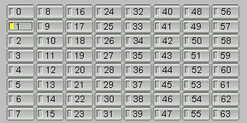
\includegraphics[scale=1]{flbutbank} 


 FLbutBank.


  A click to a button checks that button. It may also uncheck a previous checked button belonging to the same bank. So the behaviour is always that of radio-buttons. Notice that each button is labeled with a progressive number. The \emph{kout}
 argument is filled with that number when corresponding button is checked. 


 \emph{FLbutBank}
 not only outputs a value but can also activate (or schedule) an instrument provided by the user each time a button is pressed. If the \emph{iopcode}
 argument is set to a negative number, no instrument is activated so this feature is optional. In order to activate an instrument, \emph{iopcode}
 must be set to 0 or to 105 (the ascii code of character ``i'', referring to the \emph{i}
 score opcode). P-fields of the activated instrument are \emph{kp1}
 (instrument number), \emph{kp2}
 (action time), \emph{kp3}
 (duration) and so on with user p-fields. 


  The \emph{itype}
 argument sets the type of buttons identically to the \emph{FLbutton}
 opcode. By adding 10 to the \emph{itype}
 argument (i.e. by setting 11 for type 1, 12 for type 2, 13 for type 3 and 14 for type 4), it is possible to skip the current \emph{FLbutBank}
 value when getting/setting snapshots (see \emph{General FLTK Widget-related Opcodes}
). 


  FLbutBank is very useful to retrieve snapshots. 
\subsection*{See Also}


 \emph{FLbox}
, \emph{FLbutton}
, \emph{FLprintk}
, \emph{FLprintk2}
, \emph{FLvalue}

\subsection*{Credits}


 Author: Gabriel Maldonado


 New in version 4.22
%\hline 


\begin{comment}
\begin{tabular}{lcr}
Previous &Home &Next \\
FLbox &Up &FLbutton

\end{tabular}


\end{document}
\end{comment}
